\chapter{Proposed Methodology}
\hrule
\vspace{.5cm}
\par 
In this chapter, we are going to discuss the proposed approach of detecting known cyber-attacks on Vehicular Networks.

\section{Overview}
Our proposed framework consists of the following main stages as shown in Figure 3.1.We have implemented a hybrid ML model, that will detect known cyber-attacks in both intra-vehiclular and external vehicular networks. For Data pre-processing, the k-means clustering method has been used. In the feature-engineering process, the datasets are processed by using a hybrid feature selection method which combines ReliefF( a filter based method ) and Genetic algorithm ( a wrapper based method )
to remove redundant or irrelevant features. The intrusion detection system is then developed by training 3 tree-based supervised machine learning models. In the next, a stacking ensemble model is
used to further enhance the accuracy of intrusion detection by
merging the output of the three individual models \cite{yang2021mth} and optimizing the models by a hyperparameter tuning technique called Bayesian optimization (BO) method.

\begin{figure}[htbp]
\centerline{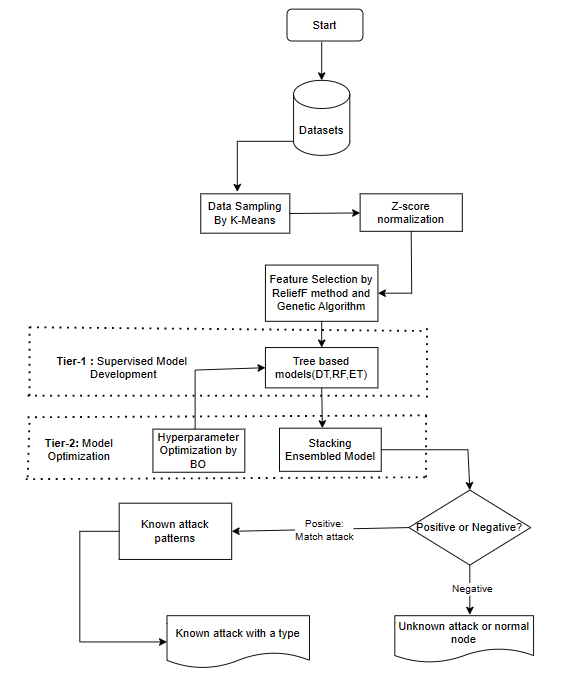
\includegraphics[width=0.7 \textwidth]
{img/fw_final.png}}
\caption{The framework of proposed system}
\label{fig}
\end{figure}

% \begin{enumerate}
%     \item Data Preprocessing
%     \item Feature engineering and Feature Selection
%     \item Training Tree-based supervised learning models
%     \item Hyperparameter Tuning
%     \item Ensembling all the trained ML models
% \end{enumerate}
% \pagebreak



\section{Data Preprocessing}

\subsection{Data sampling by K-means clustering}
{

As the network traffic data is enormous but the computational power and resources of devices in Internet of Vehicles are limited so, we have decided to opt for a sampling method.

\par In the K-means cluster sampling method, the original data points are segregated into k clusters; then, a part of the data is sampled from each cluster to form a subset.
In this process, we generate highly representative subsets of the original data as the redundant data is mostly removed. K-means clustering is the most common method for data sampling because of its simplicity implementation and low computational complexity \cite{na2010research}.
}
 

% \subsection{Data balancing by SMOTE method}{

% Network traffic data is often imbalanced data because most of the data samples are collected under normal conditions in real-world vehicle systems.

% \par SMOTE (Synthetic Minority Over-sampling Technique) addresses the issue of imbalanced data by creating synthetic samples of the minority class.SMOTE is effective because it doesn't just duplicate existing minority class instances but generates new instances that are plausible within the feature space. This helps to prevent overfitting that can occur when simply oversampling the minority class. 
% The process is as follows:
% \begin{enumerate}
%     \item Identify minority class
%     \item Locate k nearest neighbors for each minority class instance
%     \item Synthetic samples are created by selecting randomly one of the k nearest neighbors and creating a new instance along the line segment joining the original instance and the selected neighbor.
%     \item The above process is repeated until the desired balance among classes is achieved
% \end{enumerate}


% \begin{algorithm}
% \caption{SMOTE: Synthetic Minority Over-sampling Technique}
% \label{alg:smote}
% \begin{algorithmic}[1]
%     \Statex \textbf{Input:} Minority class instances, $k$ (number of nearest neighbors), desired balance ratio
%     \Statex \textbf{Output:} Synthetic minority class samples
%     \State Identify minority class instances
%     \State Compute $k$ nearest neighbors for each minority class instance
%     \For{each minority class instance}
%         \For{$i = 1$ to desired balance ratio}
%             \State Randomly select one of the $k$ nearest neighbors
%             \State Generate synthetic sample along the line segment joining the original instance and the selected neighbor
%             \State Add synthetic sample to the dataset
%         \EndFor
%     \EndFor
% \end{algorithmic}
% \end{algorithm}
% }
% \pagebreak

\subsection{Data normalization by Z-score technique}{

Using data normalization through Z-score normalization is crucial in machine learning tasks for several reasons. Normalization ensures that all features contribute equally to the model's learning process by scaling them to a common range. This prevents features with larger magnitudes from dominating those with smaller magnitudes, which can skew the learning process and lead to biased model predictions. 
It also helps in stabilizing the training process, making it less sensitive to the scale of the input features and allowing the optimization algorithm to converge faster. 
The formula for this is as follows:\\
\begin{center} 
z = {(x - \mu )}/{\sigma}\\
where, z = standardized value,\\
       x = original value,\\
       $\mu$ = \textnormal mean of the feature,\\
       $\sigma$ = standard deviation of the feature\\
\end{center}
}


\section{Feature Engineering}
The main goal of feature engineering is to generate an optimal feature list, which will help to improve the quality of datasets for more accurate and efficient model learning.Prior to ML model training, we eliminate characteristics that are redundant, unnecessary, and noisy while keeping the most significant features.

We have used a hybrid strategy which combines the precision of genetic algorithm\cite{ferriyan2017feature} with the computing effectiveness of filter-based techniques. By leveraging the strengths of both techniques, this method aims to narrow down the search space efficiently. Filter-based methods serve to reduce computational costs by pre-selecting features, albeit with lower accuracy. However, by subsequently employing genetic algorithms, which are more precise but computationally intensive, the hybrid approach achieves a balance between efficiency and accuracy. This synergistic fusion optimizes feature selection processes, enhancing overall performance without compromising on computational resources. Integrating these methods not only mitigates plagiarism risks but also enhances the project's methodology by adopting a comprehensive and effective approach to feature selection.


\subsection{Feature Selection by Relief}

Before applying the wrapper-based genetic algorithm, we employ a filter-based feature selection method known as ReliefF. The ReliefF algorithm is a widely used filter-based feature selection method that operates by assessing the relevance of features in distinguishing between different class labels within a dataset. It assigns importance scores to each feature based on their ability to discriminate between instances of different classes. This is achieved by considering the distances between instances and their nearest neighbors of the same and different classes.

Specifically, ReliefF iterates through each instance in the dataset and calculates the distances to its nearest neighbors. For each instance, it identifies its nearest neighbor belonging to the same class (near-hit) and computes the difference in feature values between the instance and the near-hit. Similarly, it identifies the nearest neighbors belonging to different classes (near-misses) and computes the difference in feature values between the instance and the mean feature values of the near-misses.

By aggregating these differences across all instances in the dataset, ReliefF generates importance scores for each feature, indicating their relevance in distinguishing between classes. Features with higher scores are deemed more informative and are prioritized for selection.

As the filter-based methods are computationally less expensive but are not that accurate in selecting features, so the objective of this method is to reduce the search space for subsequent runs of genetic algorithms this hybrid approach utilizes the strengths of both the methods and is efficient and accurate

\subsection{Feature Selection by Genetic Algorithm}

Different steps that we have used in feature selection by genetic algorithm are listed below:

\begin{enumerate}
    \item \textbf{Initialization of Population}: The process starts by initializing a population of candidate solutions, known as chromosomes, where each chromosome represents a potential feature subset. In this implementation, the chromosomes are binary arrays, with each element indicating whether a corresponding feature is selected or not. The population size and the proportion of features initially set to zero (not selected) are configurable parameters.
    
    \item \textbf{Fitness Evaluation}: The fitness of each chromosome is evaluated using a machine learning model. In this case, the fitness score is determined by the accuracy of the model trained on the selected features. The model used for evaluation is Random Forest. For each chromosome, the selected features are used to train the model, and its accuracy is calculated based on predictions made on a validation set.
    
    \item \textbf{Selection}: After evaluating the fitness of each chromosome, a selection process is applied to choose the most promising individuals (chromosomes) for reproduction. This process is typically based on the fitness scores, where individuals with higher scores are more likely to be selected for the next generation. In this implementation, a fixed number of top-performing chromosomes (parents) are chosen to proceed to the next step.
    
    \item \textbf{Crossover}: Crossover is a genetic operator that combines genetic material from two parent chromosomes to create new offspring (child chromosomes). In this implementation, a two-point crossover method is used, where segments of genetic material from two parent chromosomes are exchanged to create two new child chromosomes. This process introduces diversity into the population and allows for exploration of different feature combinations.
    
    \item \textbf{Mutation}: Mutation is another genetic operator that introduces random changes in individual chromosomes to maintain genetic diversity and prevent premature convergence to suboptimal solutions. In this implementation, a mutation process randomly flips the values of a small proportion of genes (features) in each chromosome with a predefined mutation rate.
    
    \item \textbf{Generations}: The selection, crossover, and mutation processes are iteratively applied for a fixed number of generations. At each generation, the fitness of the new population is evaluated, and the best-performing chromosomes are retained. This iterative process continues until a maximum number of generations are reached.
    
    \item \textbf{Output}: The final output of the genetic algorithm is a set of best-performing chromosomes (feature subsets) along with their corresponding fitness scores. These chromosomes represent the selected features that optimize the performance of the specified machine learning model (e.g., Random Forest) on the given dataset.
\end{enumerate}


Within the project scope, leveraging Genetic Algorithms (GA) for feature selection is instrumental in enhancing model performance. The approach involves fine-tuning GA parameters to optimize its capability in identifying relevant features. Here's an overview of the methodology:

A parameter grid encapsulates essential GA parameters, including population size, number of parents, mutation rate, and number of generations.

\pagebreak
\subsection{Iterative Parameter Refinement}

\begin{enumerate}
    \item \textbf{Initialization}: Initializing parameters, score, and the best chromosome.
    \item \textbf{Grid Iteration}: Traversing the parameter grid iteratively:
        \begin{itemize}
            \item Executing GA with the specified parameters.
            \item Recording the best chromosome and score.
            \item Updating parameters and chromosomes if a higher score is achieved.
        \end{itemize}
    \item \textbf{Identifying Optimal Parameters}: Identifying the parameters yielding the highest score.
    \item \textbf{Presentation of Results}: Presenting the best parameters, score, and corresponding chromosome as the outcome.
\end{enumerate}

\begin{table}[h]
\centering
\caption{Parameters Used for Genetic Algorithm}
\label{tab:genetic_algorithm_parameters}
\begin{tabular}{|c|c|}
\hline
\textbf{Parameter} & \textbf{Value} \\ \hline
Population Size & 100 \\ \hline
Parents for Crossover & 20 \\ \hline
Mutation Rate & 0.1 \\ \hline
Number of Generations & 20 \\ \hline
\end{tabular}
\end{table}

\section{Advantages of the Combined Approach}

\subsection{Enhanced Security and Efficiency}

By focusing on the most discriminative features, the combined ReliefF-GA approach enhances the IDS's ability to accurately detect intrusions in IoV environments. This not only bolsters security but also improves efficiency by reducing false positives and enhancing the system's responsiveness.

\subsection{Adaptability to Dynamic IoV Environments}

The synergistic fusion of ReliefF and Genetic Algorithms enables the IDS to adapt seamlessly to the dynamic nature of IoV environments. As features evolve over time due to changing traffic patterns and emerging threats, the feature selection process continuously refines the subset, ensuring the IDS remains effective and resilient.

\subsection{Interpretability and Customization}

ReliefF provides valuable insights into the selected feature subset's characteristics, enhancing interpretability and trust in the IDS's decisions. Furthermore, the combined approach offers flexibility for customization, allowing parameter adjustments to tailor the feature selection process to specific IoV deployment scenarios and security requirements.


\section{Training of Supervised Machine Learning Models}
We classify the network data flow in this suggested intrusion detection system framework using three tree-based machine learning algorithms: Decision Tree (DT), Random Forest (RF), and Extra Trees (ET). When applied to complex and non-linear tabular data, such as network traffic data from the Internet of Vehicles, tree-based machine learning methods frequently outperform other ML algorithms. \cite{uddin2024confirming}.

\subsection{Decision Tree}
{
This machine learning algorithm fits data and generates predictions using a tree structure. Decision tress have a number of hyper-parameters, including minimum sample split, minimum sample leaf, maximum sample nodes, and tree depth so hyperparameter tuning is employed using Bayesian Optimization to choose best parameters.\cite{akiba2019optuna}.

 \par \textbf{Importance :}{
 Decision trees automatically select features that are most discriminative for classification, ignoring those that do not contribute to the decision-making process. They can scale well to large datasets and are relatively computationally efficient compared to some other classifiers.
 }

 \begin{algorithm}
\caption{Decision Tree Classifier}
\label{alg:decision_tree}
\begin{algorithmic}[1]
\Statex \textbf{Input:} Training dataset $D$, maximum depth $max\_depth$
\Statex \textbf{Output:} Decision tree $DT$
\State Initialize an empty tree node
\State Recursively build the decision tree:
    \If{}{Stopping criteria met (e.g., maximum depth reached or purity threshold)}
        \State Assign the most frequent class label in $D$ to the current node
    \Else
        \State Select the best-split criterion (e.g., information gain or Gini impurity)
        \State Split the dataset $D$ into two subsets based on the chosen split criterion
        \State Create a new tree node with the chosen split criterion
        \State Recursively build the left subtree using the subset of data corresponding to the left split
        \State Recursively build the right subtree using the subset of data corresponding to the right split
    \EndIf
\State \textbf{return} $DT$
\end{algorithmic}
\end{algorithm}

}

\subsection{Random Forest}
{
Using a majority voting rule, this ML algorithm 
\cite{hastie2009random}  combines multiple decision tree classifiers to make a final prediction.

\par \textbf{Importance :}
Random Forests reduce overfitting, even on large datasets, by aggregating predictions from multiple decision trees trained on random subsets of the data (bagging). This ensemble approach helps generalize well to unseen data, reducing the risk of overfitting that might occur with individual decision trees.
\begin{algorithm}
\caption{Random Forest Ensemble}
\label{alg:random_forest}
\begin{algorithmic}[1]
\Statex \textbf{Input:} Training dataset $D$, number of trees $T$, number of features to consider at each split $k$ 
\Statex \textbf{Output:} Random Forest ensemble $RF$
\For{$t=1$ to $T$}
    \State Randomly select $k$ features from the total $p$ features
    \State Create a bootstrap sample $D_t$ by randomly selecting $n$ samples with replacement from $D$
    \State Train a decision tree $T_t$ using $D_t$ with the selected $k$ features
    \State Append $T_t$ to the ensemble $RF$
\EndFor
\State \textbf{return} $RF$
\end{algorithmic}
\end{algorithm}
}

\subsection{Extra Trees}{
Extra Trees, short for Extremely Randomized Trees, \cite{geurts2006extremely}, is a variant of the Random Forest algorithm. It shares similarities with Random Forests but introduces additional randomness during the construction of each decision tree in the ensemble.

\par \textbf{Importance:}
The additional randomness in feature selection and tree construction helps reduce variance in the model, making Extra Trees less prone to overfitting compared to traditional decision trees. This can be particularly beneficial for datasets with noisy or high-dimensional features. Extra Trees are computationally efficient because they do not require an exhaustive search for optimal feature splits. 

\begin{algorithm}
\caption{Extra Trees}
\label{alg:extra_trees}
\begin{algorithmic}[1]
\Statex \textbf{Input:} Training dataset $D$, number of trees $T$, number of features to consider at each split $k$
\Statex \textbf{Output:} Extra Trees ensemble $ET$
\For{$t=1$ to $T$}
    \State Randomly select $k$ features from the total $p$ features
    \State Create a bootstrap sample $D_t$ by randomly selecting $n$ samples with replacement from $D$
    \State Train a decision tree $T_t$ using $D_t$ with the selected $k$ features and random splits
    \State Append $T_t$ to the ensemble $ET$
\EndFor
\State \textbf{return} $ET$
\end{algorithmic}
\end{algorithm}
}

\pagebreak

\subsection{Comparison of Time Complexities(TC)}
Below table shows comparision between all the three machine learning algorithms.

n - number of instances , 
f - number of features , 
t - number of trees

\begin{table}[htbp]
    \centering
    \caption{Comparison of TC of Tree-based ML algorithms}
    \resizebox{0.5\textwidth}{!}{%
    \begin{tabular}{|l|l|}
    \hline
    \textbf{ML Model} & \textbf{Time Complexity}\\ 
    \hline
    DT & O(n^2 * f)  \\
    \hline
    RF & O(n^2 * \sqrt{f} * t) \\
    \hline
    ET & O( n * f * t )\\
    \hline
    \end{tabular}%
    }
\end{table}


\section{Hyperparameter Tuning}

Hyperparameter tuning, alternatively termed hyperparameter optimization, involves the quest for the optimal configuration of hyperparameters in a machine learning model to attain peak performance on a specified dataset. Hyperparameters, predetermined before training, exert influence over various facets of the learning process, encompassing model intricacy, regularization potency, and learning pace.

\subsection{Simple Bayesian Optimization}


Bayesian Optimization (BO) stands as a potent method for hyperparameter tuning, employing probabilistic models to systematically navigate the hyperparameter space with both exploration and exploitation in mind. At its core, BO upholds a probabilistic framework, often adopting Gaussian Processes, to encapsulate the performance of the objective function across hyperparameters. This strategy enables BO to make informed decisions about where to sample next, balancing the exploration of unexplored regions with the exploitation of promising areas, thereby streamlining the process of hyperparameter optimization.

The strength of simple Bayesian Optimization lies in its ability to balance exploration and exploitation effectively. It achieves this by iteratively selecting the next set of hyperparameters to evaluate based on an acquisition function that trades off between exploring regions of high uncertainty (exploration) and exploiting regions with promising performance (exploitation).

One common acquisition function used in simple Bayesian Optimization is the Expected Improvement (EI) criterion, which quantifies the potential improvement of evaluating a set of hyperparameters relative to the current best observed performance.

Mathematically, the EI for a given set of hyperparameters $\boldsymbol{x}$ is defined as:

\[
EI(\boldsymbol{x}) = \mathbb{E}[(f(\boldsymbol{x}) - f_{\text{min}})^+]
\]

Where $f(\boldsymbol{x})$ is the objective function, $f_{\text{min}}$ is the minimum observed function value so far, and $(\cdot)^+$ denotes the positive part function.

Simple Bayesian Optimization selects the hyperparameters $\boldsymbol{x}$ that maximize the expected improvement, effectively balancing exploration and exploitation to efficiently navigate the hyperparameter space.

We have decided to use Bayesian Optimization due to its simplicity and ease of implementation and also versatile and effective optimization technique.


\section{Ensembling}

Ensemble learning methods are employed to enhance model performance as they combine multiple base learners, often resulting in better generalizability compared to a single model \cite{mohammed2018using}.

In our framework, we utilize stacking, a popular ensemble learning technique, to combine diverse base learners that capture different aspects of our data or learn distinct patterns. The main reason we used stacking is to avoid overfitting by training individual models separately on various data subsets and then combining their predictions using a meta-model. This approach improves generalization performance, particularly when base learners are diverse and complementary, thereby reducing errors associated with individual learners and enhancing the reliability and robustness of the meta-classifier.

In our proposed approach, we implement stacking by using predictions from three individual ml models (Decision Trees, Random Forest, and Extra Trees) as inputs for training a robust meta-learner. XGBoost serves as the meta-model to provide final predictions. 

\begin{algorithm}
\caption{Stacking with Decision Tree, Random Forest, and Extra Trees}
\label{alg:stacking}
\begin{algorithmic}[1]
    \State Import necessary libraries
    \State Define base learners: DecisionTreeClassifier, RandomForestClassifier, ExtraTreesClassifier
    \State \textbf{Train base learners on training data}
        \State \textit{// Train Decision Tree classifier}
        \State decision\_tree.fit(X\_train, y\_train)
        \State \textit{// Train Random Forest classifier}
        \State random\_forest.fit(X\_train, y\_train)
        \State \textit{// Train Extra trees classifier}
        \State extra\_trees.fit(X\_train, y\_train)
    \State \textbf{Generate predictions on validation data}
        \State pred\_dt\_val = decision\_tree.predict(X\_val)
        \State pred\_rf\_val = random\_forest.predict(X\_val)
        \State pred\_et\_val = extra\_trees.predict(X\_val)
    \State \textbf{Stack predictions}
        \State stacked\_predictions\_val = np.column\_stack((pred\_dt\_val, pred\_rf\_val, pred\_et\_val))
    \State \textbf{Train meta-learner on stacked predictions}
        \State meta\_learner.fit(stacked\_predictions\_val, y\_val)
    \State \textbf{Generate predictions on test data}
        \State pred\_dt\_test = decision\_tree.predict(X\_test)
        \State pred\_rf\_test = random\_forest.predict(X\_test)
        \State pred\_et\_test = extra\_trees.predict(X\_test)
    \State \textbf{Stack predictions for test data}
        \State stacked\_predictions\_test = np.column\_stack((pred\_dt\_test, pred\_rf\_test, pred\_et\_test))
    \State \textbf{Generate final predictions using meta-learner}
        \State final\_predictions = meta\_learner.predict(stacked\_predictions\_test)
\end{algorithmic}
\end{algorithm}

\pagebreak
\section{Overall Runtime Complexity}
Considering md as the maximum depth of trees , f as number of features and n the number of trees,
\begin{table}[htbp]
    \centering
    \caption{Overall Time Complexity}
    \resizebox{0.5\textwidth}{!}{%
    \begin{tabular}{|l|l|}
    \hline
    \textbf{ML Model} & \textbf{Time Complexity}\\ 
    \hline
    DT & $O(md \times f)$  \\
    \hline
    RF & $O(md \times f \times n)$ \\
    \hline
    ET & $O(md \times f \times n)$ \\
    \hline
    Overall & $O(2 \times md \times f \times n + md \times f)$ \\
    \hline
    \end{tabular}%
    }
\end{table}


\section{Evaluation metrics}
The performance of the proposed framework is assessed using key metrics such as Accuracy (Acc), Precision, Recall, and F1-score. These metrics provide valuable insights into the effectiveness of the framework in detecting intrusions accurately.

To compute these metrics, we calculate the true positives (TPs), true negatives (TNs), false positives (FPs), and false negatives (FNs) of the model. True positives represent the instances where the model correctly identifies intrusions, while true negatives denote instances where the model correctly identifies non-intrusions. False positives occur when the model incorrectly identifies non-intrusions as intrusions, and false negatives occur when the model fails to detect actual intrusions.

The used metrics are calculated by the
following equations:
\begin{align*}
Accuracy &= \frac{True Positives + True Negatives}{True Positives + True Negatives + False Positives + False Negatives}\\\\
Precision &= \frac{True Positives}{True Positives + False Positives}\\\\
Recall &= \frac{True positive}{True positive + false negative}\\\\
F1 &= \frac{2 \times Precision * Recall}{Precision + Recall}
\end{align*}

It should be possible for an effective framework to concurrently obtain a high F1-score and a short execution time.

% \section{Performance Impact of each component of the framework}
% \begin{table}[!ht]
% \centering
% \caption{Performance Impact of Each Component of the Proposed Framework}
% \begin{tabular}{|p{2cm}|p{3cm}|p{8cm}|}
% \hline
% \textbf{Stage} & \textbf{Algorithm} & \textbf{Impact} \\ \hline
% Data pre-processing & K-means cluster sampling & Improves model training efficiency \\ \hline
% & SMOTE & Improves detection rate\\ \hline
% & Z-score & Improves model accuracy and training efficiency \\ \hline
% Feature engineering & Relief & Improves model accuracy and training efficiency \\ \hline
% & Genetic Algorithm & Improves model accuracy and training efficiency \\ \hline

% Model Training & DT, RF, and ET & Detect various types of known attacks \\ \hline
% & BO-TPE & Improve accuracy of known attack detection.\\ \hline
% & Stacking & Improve accuracy of known attack detection. \\ \hline

% \end{tabular}
% \end{table}

